%===================================== CHAP 8 =================================

\chapter{Project evaluation}
\label{ch:project_evaluation}

\section{Research phase}
\label{sec:project_evaluation-research_phase}


After the initial evaluation of the task and its requirements, it seemed more difficult than first assumed. As none of the group members had any experience writing this kind of software, a lot of time had to be dedicated to research. Building software with this size and complexity, was unlike anything taught in previous courses. Additionally, there were hundreds of pages of protocol documentation and standards, which required a lot of time to understand. Finally, there were no similar applications which implemented a message broker for specifically for WSN. All of this required time, also during the development part of the project. In total, research accounted for a large portion of the time used in the project.

\subsection{Apollo}
\label{subsec:project_evaluation-research_phase-apollo}

Two full weeks were dedicated to research Apollo. As the total time of the project was less than one semester, that was a fairly large portion of it. The positive aspect of it, was that a lot was learned from this work, and some of the aspects and good practices were carried over to the implementation.

The decision to abandon Apollo was not made until the very end. It was only then that the components of the Apollo system proved to be so complex that it failed the gate criteria. After further discussion, additional issues appeared which led to the final decision. Had the research phase been shortened, it might have resulted in the decision to further develop Apollo, possibly resulting in a failure to deliver a working product. Thus, abandoning Apollo was probably the best choice.

\subsection{Process Model}
\label{subsec:project_evaluation-research_phase-process_model}

Although none of the group members had any experience with the phase-gate model, the choice worked out fairly well. Mainly because the first occurrence of an issue or problem that failed to meet the gate criteria would terminate further research. Subsequently, a deadline for a final decision was set, providing a firm point in time to be used in the overall project plan. This was key, as extending the research further, could potentially have had a negative impact on the development part of the project. Additionally, splitting the research work into different areas, proved effective. It caused each member to have deep insight into one area, instead of all members having some insight into everything. The negative aspect of this is that it was challenging to have technical discussions with other group members.

The parallel research approach required frequent updates internally. Since each group member had a particular area of research, structured communication was key to keep the group sufficiently updated on current progress. Each member had to work in a structured manner, considering one task at a time, and continuously log progress and results.

\subsection{Evaluation}
\label{subsec:project_evaluation-research_phase-evaluation}

The outcome of the research phase wasn't exactly as hoped. The ideal path would have been to be able to proceed with Apollo. However, the knowledge the group gained from Apollo was quite extensive, and will be useful for the customer in further research and development. The research also helped in structuring the implementation. Although a lot of time was used on Apollo, researching existing solutions is an important aspect of any development project. It was also the part of the project in which the members learned the most. Not just about Apollo and doing research work, but it was a new aspect of team work. All in all, the research work was important in order to develop a best possible solution.

Looking back at the effectiveness of the model, it proved applicable for this kind of work. In a theoretical situation, where problems might have arose at an earlier point in time, the true effectiveness of the model would have been demonstrated. However, as previously stated, this did not occur until the end of the research phase.

In retrospective, the research period should have been compressed. By starting the research period earlier, and by working more during the period, it might have been possible to cut one week of the research period. This is the most important aspect that could have been done differently. It would have led to more time available for development.

\section{Development}
\label{sec:project_evaluation-development}

Due to the research work, the development started in late February. This was a challenge, as less of the total time could be allocated to development. When constructing the development plan, the group realized that in order to complete the project, it was necessary to develop until late may. This was obviously a risk, as there would be no time to spare if something were to go wrong towards the end. Some of the less important protocols were also removed as requirements, in order to have the time to implement the most important parts.

\subsection{Process model}
\label{subsec:project_evaluation-development-process_model}

Initially, it was decided to use test-driven development. This worked out well on the parts of the system which had a clearly defined behaviour. In that regard, the model proved successful as it made the actual code writing simpler. It was however, difficult to enforce on other parts of the system. In the end, TDD weren't a huge success, as time were spent planning how to write tests, instead of using that time to develop. Thus, the group weren't able to fully achieve the advantages of the model. 

Scrum worked out well. The most important part of it was the meetings, as they helped in keeping track of progress at all times. Communication was key to assess the different development issues faced. Additionally, any problems regarding development were discussed, and assessed by the group as a whole. 

A backlog chart (task list) and burndown chart were created each sprint. The templates were initialized at the start of each sprint, and the workload were decided and distributed amongst the group. This worked out very well, as each member had clearly defined tasks for each sprints. Additionally, it was helpful to keep track of the time usage, when evaluating each sprint. The evaluation of the previous sprint were taken into consideration when defining the next. This were a helpful to assign an appropriate workload for each sprint.

Having sprints lasting two weeks were appropriate. As the group had to consider other courses and tasks, the work load varied from week to week. Thus, it was nice to have two weeks to complete the tasks assigned. Additionally, shorter sprint intervals would have led to more time being used on management of tasks and time, as it would have to be done each week. Having longer sprints could have affected the communication with the customer in a negative way. If something were implemented in a way that weren't satisfiable, it would have led to more time being used before the proper feedback were acquired. One example is the initial research made on MQTT, after it was decided that only two protocols would be implemented. At that time, it was important to know that AMQP was more important, to avoid too much time loss.

\subsection{Resource management}
\label{subsec:project_evaluation-development-time_management}

Time-estimation was one of the most difficult tasks of the project. This was partially due to the uncertainty around how much time it would take to implement protocols. The task proved way more time-consuming than the initial expectations. Additionally, the amount of research required to understand the protocols, and how to implement them were more than what was estimated.

During the development period, less time was used on development than what was planned. First of all, other courses took up a lot of time, and was not properly planned for. The group weren't able to properly structure the work days, and thus tasks in other courses hindered development at times. This could have been considered in a better way, by following the risk analysis and plan further ahead of time. Another factor were short term absence of group members. Although these factors were accounted for in the risk analysis, the issues that occurred weren't properly handled. The workload should have been distributed, and extra work hours introduced. However, it wasn't done in the majority of cases. The consequence of this was that a lot more time had to be used towards the end. The major lesson learned was to not neglect the risk analysis, and to follow up on time and resource issues that occur. 

Combining report writing and development proved to be an issue. Although all of the group members contributed to both, it was difficult to keep track of both at the same time. That led to the person responsible for report and documentation doing a lot of work on the report. While this worked out well for the process parts of the report, he did not have as much insight into the development. Thus, it was difficult to write about the actual product. Although distributing the different parts of the report was done eventually, it should have been done earlier. This would have led to steadier progress on the report. Work distribution could have been planned better, and is one of the lessons learned.

\subsection{Evaluation}
\label{subsec:project_evaluation-development-evaluation}

Overall, the development period worked out fairly well. The main issues were with resource and time management. Not enough work was devoted to the project in the early stages of the process. This proved to be an issue later on, especially due to the task being more difficult than the initial assessment. Although this was sub-optimal, the issue was solved by adding more hours towards the end of the project. Less emphasis were put on test-driven development as the project went on, but it didn't affect the product in a considerable way. Apart from that, the process model and methodology worked well. Below is a diagram showing the work distribution among the major tasks.

\begin{center}
  \begin{figure}[ht!]
    \makebox[\textwidth]{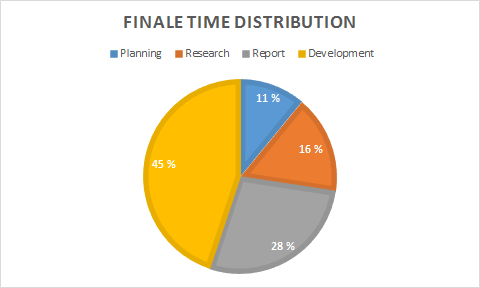
\includegraphics[width=0.9\textwidth]{fig/kake2.png}}
    \caption{Final time distribution}
    \label{fig:kake2}
  \end{figure}
\end{center}

\begin{center}
  \begin{figure}[ht!]
    \makebox[\textwidth]{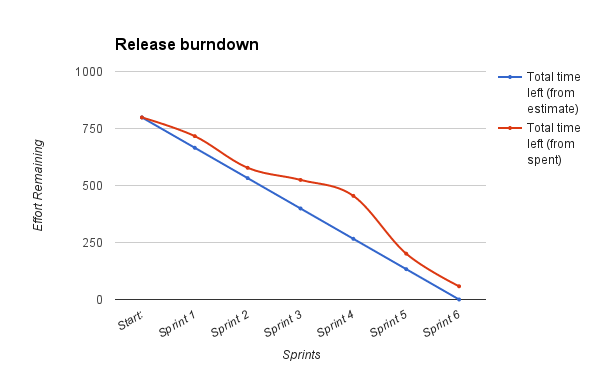
\includegraphics[width=\textwidth]{fig/burndown/releaseBurndown.png}}
    \caption{Release burndown chart}
    \label{fig:release-burndown}
  \end{figure}
\end{center}

\section{Social and cooperation aspects}
\label{sec:Social_and_cooperation_aspects}

The dynamic of the group were well. No social issues arose, and a nice work environment were upheld throughout the project. Eating lunch together, and taking breaks to talk about other things than the project made the days enjoyable. The social aspect helped throughout the project, as it kept the moral of the group high. There were some minor arguments during the development phase. These were mainly due to different opinions on code principles, report structure etc. None of these arguments led to any anger or issues between anyone in the group however.

Cooperation worked out well throughout the project, both within the group, and with the customer and supervisor. It was easy to ask questions to other members, which was helpful if someone was stuck on a specific task or problem. Additionally, group meetings functioned as an arena were more complex tasks could be assessed by the whole group. All this made development more efficient, as it often prevented long periods of time being used on a specific problem. Meeting agendas were key when communicating with the customer and supervisor. Having them provided a simple way of structuring each meeting, which made sure nothing was forgotten or neglected.

The group also occasionally talked with other groups. The discussions were mainly about status on each groups project, and occasionally helping each other with report structure. The insight into other groups were helpful, as the group had someone to compare work with. This was sort of an additional safety net, to make sure no important parts of the project were neglected.

\section{Implementation}
\label{sec:Implementation}

The group were satisfied with how the system turned out. It does what it was supposed to do and performs well, with no bottlenecks. The code is structured and documented in a good way, and modularized to make it as simple as possible to extend the system. There are still some small issues with the broker, but the main functionality is in place. 

\subsection{Web technologies}
\label{subsec:Web_technologies}

Several development tools and libraries were used in the Java implementation. Bootstrap and jQuery generally made it simpler and less time-consuming to build the web application. Bootstrap also made it simple to give the site a clean and intuitive design. 

In retrospect, the group learned that the use of WebSockets \cite{web-sockets} would have been a better approach for the administration interface. The system is now designed with AJAX for real-time update of content. It's not very scalable, and may result in high server load. Using WebSockets for this purpose would have proven much more efficient. Similar to the publish/subscribe pattern, WebSockets notify clients on a state change, instead of the clients constantly asking the server for the newest state. WebSockets wouldn't make AJAX obsolete but it would have been a better solution for serving true real-time update of content. AJAX would still have been used for making short-lived web service calls (e.g. HTTP DELETE requests). \\


\subsection{Broker}
\label{subsec:Implementation_broker}
[(--Skriv om brokerting, wsnu osv. Hva var bra, hva manglet? --)]

\subsection{AMQP}
\label{subsec:Implementation_AMQP}

[!!!!VET IKKE HVA VI SKAL GJØRE MED DET SOM STÅR HER!!!!!!!!!!!]

During the first iteration of AMQP implementation, some challenges were uncovered. The largest one was the handling of topic and queues. As a queue is a different concept compared to a topic, the implemented solution gave the user an option to choose which solution to use. Implementing Simple Authentication and Security Layer (SASL) support for authentication was another issue that proved difficult. The solution was to let the user choose whether or not to use it.

Another challenge regarding the construction of outgoing AMQP messages, was to convert a Java object to a fixed size byte array. As AMQP is a byte level protocol, this had to be resolved. The solution was to as accurately as possible calculate the objects byte size. This was done using qualified guessing by looking at the different parts of the object. After a lot of testing, the final guess only missed with between 6-12 bytes. The final size of an object was found by trial and error.

After the finalization of AMQP, the testing of the protocol implementation revealed to be more difficult than first thought. Finding applications that implements the 1.0 standard was difficult. FFI provided a version of NFFIPlayer (see section \ref{subsec:prestudies-existing_solutions-micro_wsn_and_nffiplayer}) with AMQP which implemented the 0.9.1 standard. However, due to the significant changes in the standard, it could not be used to any extent.

To be able to test the implementation properly, a functioning implementation was required. Two AMQP 1.0 Java implementations were found, and simple scripts were written to test both send and receive functionality. As there was a limited amount of free/open implementations, the group ended up using one open source solution from Apache Qpid (not proton) \cite{apache-qpid} and one commercial from SwiftMQ \cite{swift-mq}. By using these implementations, the basis for stating the correctness of the implementation and the quality of the product was solid.

\clearpage